\documentclass{article}
\usepackage[english]{babel}
\usepackage{mathtools}
\usepackage{../lib/tex/naproche}
\documentclass[12pt,oneside]{book}

\usepackage[foundations]{../../lib/tex/naproche}
\usepackage{../../lib/tex/libraries}
\usepackage{graphicx}
\usepackage{float}
\usepackage{caption}
\usepackage{footnote}

\makesavenoteenv{tabular} % Make footnotes work in tabular environments


\title{Foundations of Mathematics}
\author{Marcel Schütz}
\date{2022}

\begin{document}
  \maketitle

  \tableofcontents

  \begin{figure}[H]
    \centering
    \fbox{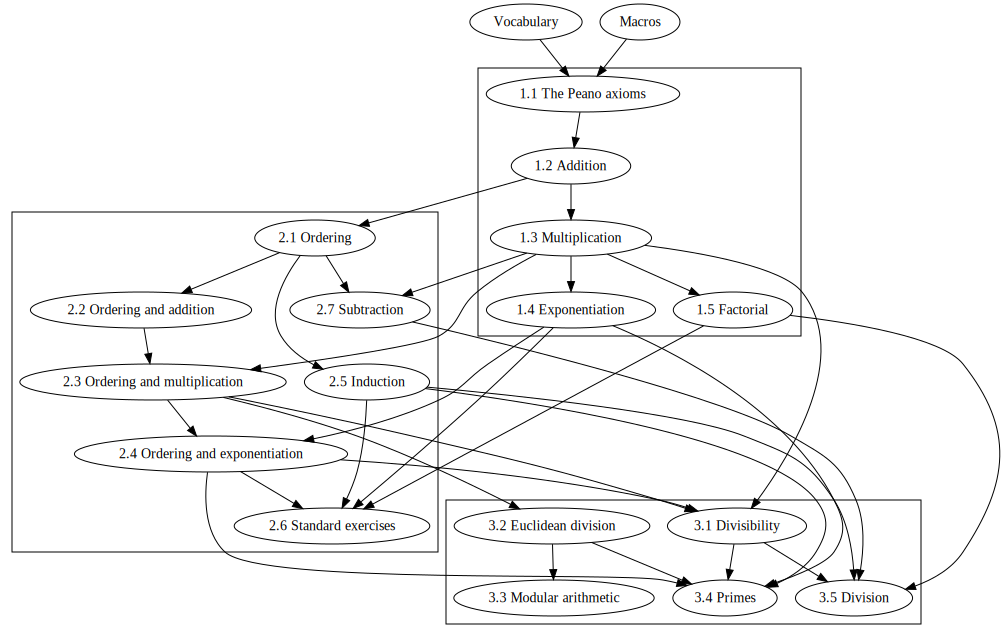
\includegraphics[width=0.9\linewidth]{./dependency-graph/graph.png}}
    \caption*{Interdependencies of the chapters}
  \end{figure}


  \section*{Introduction}

  This is a library providing a foundation of mathematics based on a
  Kelley-Morse like class theory with urelements.
  It introduces common operations on classes like unions or intersections
  (\cref{chapter:classes}) together with detailed proofs of their algebraic
  properties (\cref{chapter:computation-laws-for-classes}), the symmetric
  difference of two classes (\cref{chapter:symmetric-difference}) and the
  notions of ordered pairs and Cartesian products
  (\cref{chapter:pairs-and-products}) as well as proofs of the algebraic
  properties of the latter (\cref{chapter:computation-laws-for-products}).
  Moreover, it provides common operations on maps (\cref{chapter:maps}), various
  properties of images and preimages (\cref{chapter:image-and-preimage}) and the
  notions of injectivity, surjectivity, bijectivity
  (\cref{chapter:injections-surjections-bijections}) and invertibility of maps
  (\cref{chapter:invertible-maps}).
  The library provides an axiom system characterizing sets (\cref{chapter:sets})
  and, furthermore, it covers the notions of binary relations
  (\cref{chapter:binary-relations}), fixed-points of subset preserving maps
  (\cref{chapter:fixed-points}), including and equinumerosity
  (\cref{chapter:equinumerosity}).

  As two famous results it includes the Knaster-Tarski fixed point theorem
  (\cref{FOUNDATIONS_12_8420450166112256}) and the Cantor-Schröder-Bernstein
  theorem (\cref{FOUNDATIONS_13_1913663275401216}).

  \paragraph*{Usage.}
  At the very beginning of each chapter you can find the name of its source
  file, e.g. \path{foundations/sections/01_classes.ftl.tex} for
  \cref{chapter:classes}. This filename can be used to import the chapter via
  \Naproche's \texttt{readtex} instruction to another ForTheL text, e.g.:
  \begin{center}
    \verb`[readtex \path{foundations/sections/01_classes.ftl.tex}]`
  \end{center}

  \paragraph*{Checking times.}
  The checking times for each of the chapters may vary from computer to
  computer, but on mid-range hardware they are likely to be similar to those
  given in table below:

  \begin{center}
    \begin{tabular}{c|c|c}

      & \multicolumn{2}{c}{\textbf{Checking time}}
      \\
      \textbf{Chapter}
      & \textbf{without dependencies}     & \textbf{with dependencies}
      \\ \hline
      \ref{chapter:classes}
      & 00:04 min                         & 00:04 min
      \\
      \ref{chapter:computation-laws-for-classes}
      & 00:12 min                         & 00:16 min
      \\
      \ref{chapter:symmetric-difference}
      & 00:32 min                         & 00:48 min
      \\
      \ref{chapter:pairs-and-products}
      & 00:08 min                         & 00:12 min
      \\
      \ref{chapter:computation-laws-for-products}
      & 01:36 min                         & 01:56 min
      \\
      \ref{chapter:maps}
      & 01:13 min                         & 01:25 min
      \\
      \ref{chapter:image-and-preimage}
      & 01:28 min                         & 02:53 min
      \\
      \ref{chapter:injections-surjections-bijections}
      & 00:38 min                         & 02:03 min
      \\
      \ref{chapter:invertible-maps}
      & 02:20 min                         & 04:23 min
      \\
      \ref{chapter:sets}
      & 02:17 min                         & 06:40 min
      \\
      \ref{chapter:binary-relations}
      & 00:14 min                         & 06:54 min
      \\
      \ref{chapter:fixed-points}
      & 00:33 min                         & 07:13 min
      \\
      \ref{chapter:equinumerosity}
      & 01:48 min                         & 09:01 min
    \end{tabular}
  \end{center}


  \subfile{sections/01_classes.ftl.tex}
  \subfile{sections/02_computation-laws-for-classes.ftl.tex}
  \subfile{sections/03_symmetric-difference.ftl.tex}
  \subfile{sections/04_pairs-and-products.ftl.tex}
  \subfile{sections/05_computation-laws-for-products.ftl.tex}
  \subfile{sections/06_maps.ftl.tex}
  \subfile{sections/07_image-and-preimage.ftl.tex}
  \subfile{sections/08_injections-surjections-bijections.ftl.tex}
  \subfile{sections/09_invertible-maps.ftl.tex}
  \subfile{sections/10_sets.ftl.tex}
  \subfile{sections/11_binary-relations.ftl.tex}
  \subfile{sections/12_fixed-points.ftl.tex}
  \subfile{sections/13_equinumerosity.ftl.tex}
\end{document}

\documentclass[12pt,oneside]{book}

\usepackage[utf8]{inputenc}
\usepackage[english]{babel}

\usepackage{../meta-inf/lib/naproche-logo}
\usepackage{../meta-inf/lib/naproche}
\usepackage{../meta-inf/lib/libraries}
\usepackage{naproche}
\usepackage{naproche-libraries}
\renewcommand\libarchive{Preliminaries}
\usepackage{naproche}
\usepackage{naproche-libraries}
\renewcommand\libarchive{Preliminaries}

\usepackage{xr}
\externaldocument{../foundations/foundations}

\usepackage{graphicx}
\usepackage{float}
\usepackage{caption}
\usepackage[nobottomtitles]{titlesec}


\title{Set theory}
\author{Marcel Schütz}
\date{2022}

\begin{document}
  \maketitle

  \tableofcontents

  \paragraph*{}
  \begin{figure}[H]
    \centering
    \fbox{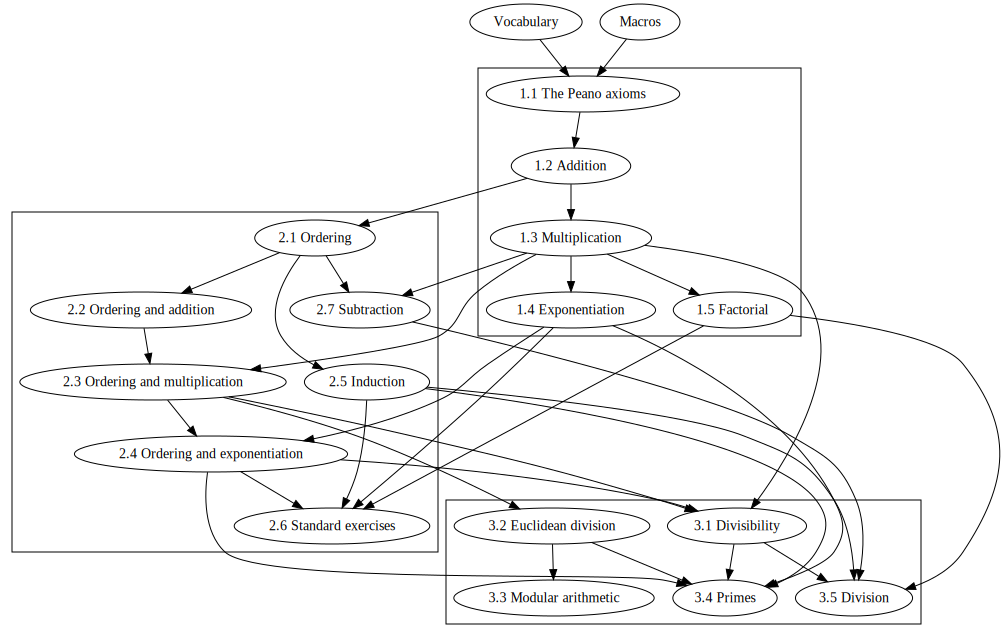
\includegraphics[width=0.9\textwidth]{./dependency-graph/graph.png}}
    \caption*{Interdependencies of the chapters}
  \end{figure}

  \section*{Introduction}

  This is a library providing basic results from undergraduate-level set theory.
  It introduces the notion of transitive classes
  (\cref{chapter:transitive-classes}), defines the notion of ordinal numbers
  (\cref{chapter:ordinals}) and as a special case of the latter introduces the
  set $\omega$ of finite ordinals (\cref{chapter:finite-ordinals}).
  Moreover, this library provides a formalization of the ordinal recursion
  theorem (\cref{chapter:recursion}) which is used to prove Zermelo's
  well-ordering theorem (\cref{chapter:zermelo}), on the basis of which the
  notion of cardinal numbers is introduced (\cref{chapter:cardinals}).
  Furthermore, some results about finite and infinite sets are given
  (\cref{chapter:finite-and-infinite-sets}).

  \paragraph*{Usage.}
  At the very beginning of each chapter you can find the name of its source
  file, e.g. \path{set-theory/sections/01_transitive-classes.ftl.tex} for
  \cref{chapter:transitive-classes}.
  This filename can be used to import the chapter via \Naproche's
  \texttt{readtex} instruction to another ForTheL text, e.g.:
  \begin{center}
    \verb`[readtex \path{set-theory/sections/01_transitive-classes.ftl.tex}]`
  \end{center}

  \paragraph*{Checking times.}
  The checking times for each of the chapters may vary from computer to
  computer, but on mid-range hardware they are likely to be similar to those
  given in table below:

  \begin{center}
    \begin{tabular}{c|c|c}

      & \multicolumn{2}{c}{\textbf{Checking time}}
      \\
      \textbf{Chapter}
      & \textbf{without dependencies}     & \textbf{with dependencies}
      \\ \hline
      \ref{chapter:transitive-classes}
      & 00:20 min                         & 07:00 min
      \\
      \ref{chapter:ordinals}
      & 03:20 min                         & 10:30 min
      \\
      \ref{chapter:finite-ordinals}
      & 01:15 min                         & 11:45 min
      \\
      \ref{chapter:recursion}
      & 04:05 min                         & 14:35 min
      \\
      \ref{chapter:zermelo}
      & 04:45 min                         & 21:40 min
      \\
      \ref{chapter:cardinals}
      & 05:10 min                         & 26:50 min
      \\
      \ref{chapter:finite-and-infinite-sets}
      & 10:50 min                         & 38:55 min
    \end{tabular}
  \end{center}

  \subfile{sections/01_transitive-classes.ftl.tex}
  \subfile{sections/02_ordinals.ftl.tex}
  \subfile{sections/03_finite-ordinals.ftl.tex}
  \subfile{sections/04_recursion.ftl.tex}
  \subfile{sections/05_well-ordering-theorem.ftl.tex}
  \subfile{sections/06_cardinals.ftl.tex}
  \subfile{sections/07_finite-and-infinite-sets.ftl.tex}
\end{document}


\usepackage[backend=bibtex]{biblatex}
\usepackage{csquotes}
\addbibresource{meta-inf/lib/bibliography}

\title{König's Theorem}
\author{\Naproche formalization: \vspace{0.5em} \\
Steffen Frerix and Peter Koepke \\
University of Bonn}
\date{2018 - 2021}

\newcommand{\SumSet}[2]{\bigsqcup_{i \in #2} #1_{i}}
\newcommand{\Sum}[2]{\sum_{i \in #2} #1_{i}}
\newcommand{\ProdSet}[2]{\bigtimes_{i \in #2} #1_{i}}
\newcommand{\Prod}[2]{\prod_{i \in #2} #1_{i}}


\begin{document}

\maketitle

\noindent König's Theorem is an important set-theoretical result about the
arithmetic of cardinals.
It was proved by Julius König in 1905 \cite[p. 177--180]{Koenig1905}.
The proof is reminiscent of Cantor's diagonal argument for proving that
$\kappa < 2^\kappa$.

\begin{imports}
  \begin{forthel}
    %[prove off][check off]
    [readtex \path{libraries/source/set-theory/cardinals-and-maps.ftl.tex}]
    %[prove on][check on]
  \end{forthel}
\end{imports}


\section*{Sums and Products of cardinals}

\begin{forthel}
  Let $f_{i}$ stand for $f(i)$.
  Let $D$ denote a set.

  \begin{definition*}
    A sequence of cardinals on $D$ is a function $\kappa$ such that
    $\dom(\kappa) = D$ and $\kappa_{i}$ is a cardinal for every element $i$ of $D$.
  \end{definition*}

  \begin{definition*}
    Let $\kappa$ be a sequence of cardinals on $D$.
    \[ \SumSet{\kappa}{D} = \class{(n,i) | \text{$i$ is an element of $D$ and $n$ is an element of $\kappa_{i}$}}. \]
  \end{definition*}

  \begin{axiom*}
    Let $\kappa$ be a sequence of cardinals on $D$.
    Then $\SumSet{\kappa}{D}$ is a set.
  \end{axiom*}

  \begin{definition*}
    Let $\kappa$ be a sequence of cardinals on $D$.
    \[ \Sum{\kappa}{D} = \left| \SumSet{\kappa}{D} \right|. \]
  \end{definition*}

  \begin{definition*}
    Let $\kappa$ be a sequence of cardinals on $D$.
    \[ \ProdSet{\kappa}{D} = \class{f | \classtext{$f$ is a function and $\dom(f) = D$ and $f(i)$ is an element of $\kappa_{i}$ for every element $i$ of $D$}}. \]
  \end{definition*}

  \begin{axiom*}
    Let $\kappa$ be a sequence of cardinals on $D$.
    Then $\ProdSet{\kappa}{D}$ is a set.
  \end{axiom*}

  \begin{definition*}
    Let $\kappa$ be a sequence of cardinals on $D$.
    \[ \Prod{\kappa}{D} = \left| \ProdSet{\kappa}{D} \right|. \]
  \end{definition*}
\end{forthel}

König's Theorem requires some form of the axiom of choice.
Currently choice is built into Naproche by the \emph{choose} construct in
function definitions.
The axiom of choice is also required to show that products of non-empty factors
are themselves non-empty:

\begin{forthel}
  \begin{lemma*}[Choice]
    Let $\lambda$ be a sequence of cardinals on $D$.
    Assume that $\lambda_{i}$ has an element for every element $i$ of $D$.
    Then $\ProdSet{\lambda}{D}$ has an element.
  \end{lemma*}
  \begin{proof}
    Define $f(i) =$ ``choose an element $v$ of $\lambda_{i}$ in $v$'' for $i$in $D$.
    Then $f$ is an element of $\ProdSet{\lambda}{D}$.
  \end{proof}
\end{forthel}


\section*{König's theorem}

\begin{forthel}
  \begin{theorem*}[König]\label{koenig}
    Let $\kappa, \lambda$ be sequences of cardinals on $D$.
    Assume that for every element $i$ of $D$ $\kappa_{i} < \lambda_{i}$.
    Then \[ \Sum{\kappa}{D} < \Prod{\lambda}{D}. \]
  \end{theorem*}
  \begin{proof}[by contradiction]
    Assume the contrary.
    Then \[ \Prod{\lambda}{D} \leq \Sum{\kappa}{D}. \]
    Take a surjective map $G$ from $\SumSet{\kappa}{D}$ to $\ProdSet{\lambda}{D}$.
    Indeed $\ProdSet{\lambda}{D}$ and $\Sum{\kappa}{D}$ are nonempty sets.
    Take $\Lambda = \bigcup \range(\lambda)$.
    Then $\Lambda$ is a set.
    Indeed $\range(\lambda)$ is a set.

    $(n,i) \in \dom(G)$ for every $i \in D$ and every $n \in \kappa_{i}$.
    $G(n,i) \in \ProdSet{\lambda}{D}$ for every $i \in D$ and every $n \in \kappa_{i}$.
    Hence for every $i \in D$ and every $n \in \kappa_{i}$ $G(n,i)$ is a map such that $i \in \dom(G(n,i))$.

    Define $\Delta(i) = \{ G(n,i)(i) \in \Lambda \mid n \in \kappa_{i} \}$ for $i \in D$.

    For every element $f$ of $\ProdSet{\lambda}{D}$ and every element $i$ of $D$ we have $f(i) \in \Lambda$.

    For every element $i$ of $D$ we have $|\Delta(i)| < \lambda_{i}$. \\
    Proof.
      Let $i$ be an element of $D$.
      Define $F(n) = G(n,i)(i)$ for $n$ in $\kappa_{i}$.
      Then $F$ is a map from $\kappa_{i}$ to $\lambda_{i}$.
      We have $\Delta(i) = \{ F(n) \mid n \in \kappa_{i} \}$.
      Thus $F[\kappa_{i}] = \Delta(i)$.
      Therefore $|\Delta(i)|
        = |F[\kappa_{i}]|
        \leq |\kappa_{i}|
        = \kappa_{i}
        < \lambda_{i}$.
      Indeed $|F[\kappa_{i}]| \leq |\kappa_{i}|$ (by \printref{SET_THEORY_06_8113916590686208}).
      Indeed $\kappa_{i}$ and $\lambda_{i}$ are sets.
    End.

    Define $f(i) =$ ``choose an element $v$ of $\lambda_{i} \setminus \Delta(i)$ in $v$'' for $i \in D$.
    Indeed $\lambda_{i} \setminus \Delta(i)$ is nonempty for each $i \in D$.
    Then $f$ is an element of $\ProdSet{\lambda}{D}$.
    Take an element $j$ of $D$ and an element $m$ of $\kappa_{j}$ such that $G(m,j) = f$.
    $G(m,j)(j)$ is an element of $\Delta(j)$ and $f(j)$ is not an element of $\Delta(j)$.
    Contradiction.
  \end{proof}
\end{forthel}

\printbibliography
\end{document}
